\chapter{Quantum physics}
\section{Photoelectric effect}
\begin{definition}{Photoelectric effect}{photoelectric}
	Phenomenon in which (photo)electrons are liberated from a \it{cool metal surface}
	when \it{e.m.~radiation} of sufficiently high frequency is incident on it.
\end{definition}
\begin{definition}{Work function}{work-func}
	\(\phi\), minimum amount of energy required to remove an electron from the metal surface.
	\vspace*{.5em}
	\footnotesize This property is intrinsic to the metal.
\end{definition}
\begin{definition}{Threshold frequency}{f-naught}
	\(f_0\), minimum frequency of the electromagnetic radiation
	required to liberate photoelectrons from a metal surface.
	\[\phi = hf_0\]
\end{definition}

Electromagnetic radiation exists in quanta---\term{photons}:
\begin{definition}{Photon}{photon}
	A discrete packet or \it{quantum} of energy of e.m.~radiation. Its energy \(E\) is
	\[E = hf = \lf{hc}{\lambda}\]
\end{definition}

Each photon--electron interaction is \it{one-to-one}: energy of one photon
is either fully absorbed by one electron, or not at all.

The photoelectric effect proves that light is quantised, by observing:
\begin{itemize}
	\item electrons emitted iff \(f_\text{incident} \geq f_0\) (threshold frequency), regardless of intensity
	\item maximum k.e.~of emitted electrons \(\propto\) frequency of incident light, regardless of intensity
	\item maximum k.e.~of emitted electrons independent of intensity of incident light
	      \[K_{\max}= h f_{\text{photon}} - \phi\]
	\item rate of emission of photoelectrons \(\propto\) intensity of incident light
	      \[\text{intensity}\times\text{area} = P = \f{E}{t} = \f{n_{\ce{e-}}}{t}\times{hf}\]
\end{itemize}

\section{Diffraction and interference}
\begin{marginfigure}
	\centering
	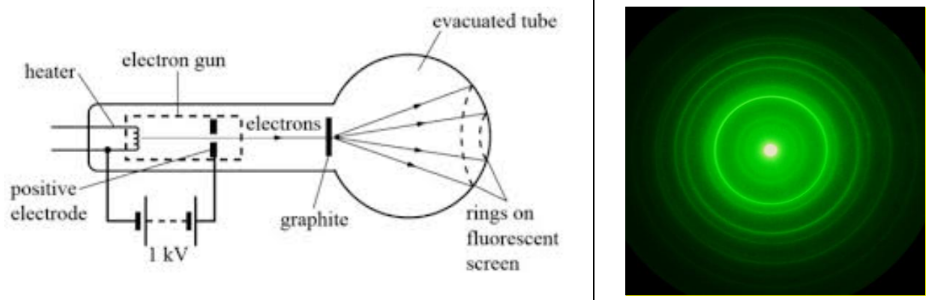
\includegraphics[width=\textwidth]{assets/e-diffraction.png}
	\caption{Diffraction experiment; diffraction pattern of \ce{e-}}
	\label{fig:e-diffraction}
\end{marginfigure}
The diffraction pattern of an electron beam contains
\it{concentric rings} with \it{alternating bright and dark regions}.

\(\implies \)\hil{\ce{e-} exhibit wave-like behaviour.}

As such, the electrons must be associated with a \it{wavelength}, with
the same order of magnitude as the crystal's atomic spacing.

\(\implies\) \hil{\ce{e-} in motion have an associated \(\lambda\).}

\begin{marginfigure}
	\centering
	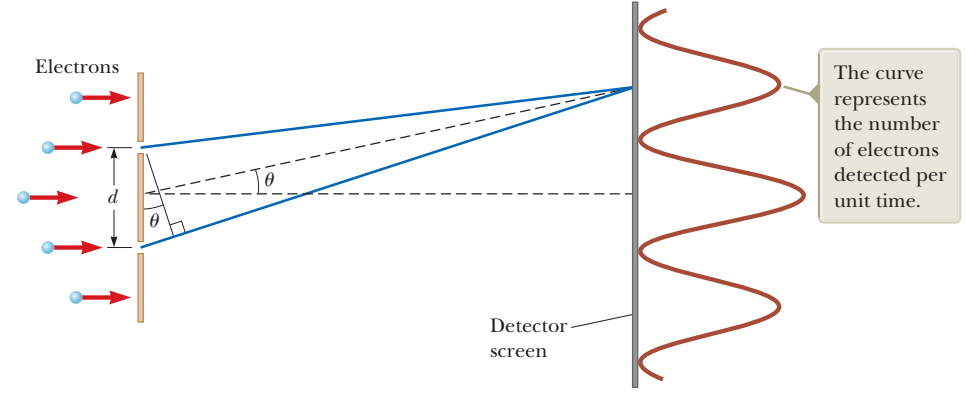
\includegraphics[width=\textwidth]{assets/e-double-slit.png}
	\caption{Double slit experiment}
	\label{fig:e-double-slit}
\end{marginfigure}
Over time, the accumulated detections form a pattern
resembling Young's double slit. High \ce{e-} density regions
correspond to \it{constructive interference}; low \ce{e-} density
regions correspond to \it{destructive interference}.

\(\implies\) \hil{\ce{e-} possess wave-like properties.}

\begin{definition}{Wave-particle duality}{wp-duality}
	The principle that \it{neither the wave or particle model alone} is sufficient
	to describe microscopic systems.
	\\\footnotesize
	Both e.m.~radiation and matter exhibit \it{wave-like and particle-like behaviour}.
\end{definition}

Photons have \term{momentum}, which can be associated with its de Broglie \term{wavelength}.
\[p = \f{E}{c} = \f{h}{\lambda}\]
\hil{Wave-like behaviour is due to a particle's motion}.

\section{Wave-like behaviour}
The \term{wavefunction} \(\psi\ab(x)\) describes the waveform
formed by matter/radiation. It must satisfy the conditions:
\begin{itemize}
	\item \(\psi\ab(x)\) must be continuous and oscillatory
	\item \(\psi\ab(x)\) must be normalisable, s.t.~\(\int_{-\infty}^{+\infty} {\ab|\psi\ab(x)|}^2 \odif{x}=1\)
	\item \(\psi\ab(x)\to 0\) as \(x\to\pm\infty\), total probability must be finite
\end{itemize}

\begin{definition}{Probability density function}{pdf}
	The probability of finding a particle (e.g.~electron, photon) at a position \(x\).
	It is the square of the amplitude of the wavefunction.
	\[\text{pdf} \coloneq {\ab|\psi\ab(x)|}^2\]
\end{definition}

The probability of finding a particle within a region of width \(\Delta x\) is then \(\text{proba} = {\ab|\psi\ab(x)|}^2\cdot\Delta x\).

The probability of finding a particle within a region \(a\leq x\leq b\) is
\[\int_a^b {\ab|\psi\ab(x)|}^2\odif{x}\]

\section{Heisenberg uncertainty principle}
\begin{definition}{Heisenberg uncertainty principle}{heisenberg}
	\[\Delta x \Delta p_x \geq h\]
	A particle's position and momentum cannot both be sharply defined.
\end{definition}

For a wave packet to be \it{localised} in position (i.e.~confined within a certain \(\Delta x\)),
waves of a large range of wavelengths \(\Delta\lambda\) must be superposed.
Spread in \(\lambda\) \(\implies\) spread in \(p\), by \(p=\lf{h}{\lambda}\).

For a wave packet have a perfectly defined \(\lambda\) (i.e.~perfectly defined \(p\)),
it must be a single infinite wave extending over space (i.e.~\it{delocalised}), hence
\(\Delta x\) is large.

\section{Quantisation of energy}
\subsection{Particle-in-box}
\begin{marginfigure}
	\centering
	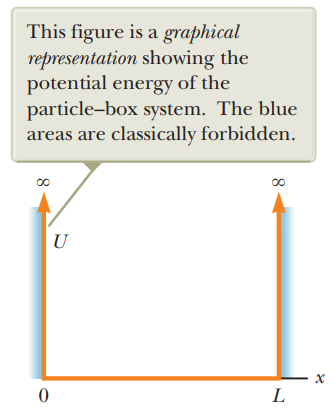
\includegraphics[width=0.75\textwidth]{assets/particle-in-box-u.png}
	\caption{\(U\ab(x)\) for particle in box}
	\label{fig:particle-in-box-u}
\end{marginfigure}
Confine a particle that only possesses k.e.~\(K\) in a box
spanning \(0\leq x\leq L\). Since the particle has no potential energy,
\begin{equation*}
	U\ab(x) = \begin{cases}
		0      & 0\leq x \leq L   \\
		\infty & \text{otherwise}
	\end{cases}
\end{equation*}
Whatever wavefunction \(\psi\ab(x)\) the particle follows must satisfy \it{boundary conditions}, since
it cannot be found outside the box:
\[\psi\ab(x=0)=0,\quad\psi\ab(x=L)=0\]

Since the particle is \it{free}, it can form \it{stationary waves} in the box. For the standing wave
to fit exactly in the box, the box must contain an integer number of segments (length \(\lf{\lambda}{2}\)):
\[L=\lf{n\lambda}{2} \implies \lambda_n = \lf{2L}{n}\]
\hil{The particle can only take on \it{allowed wavelengths}.}

\begin{figure}[htpb]
	\centering
	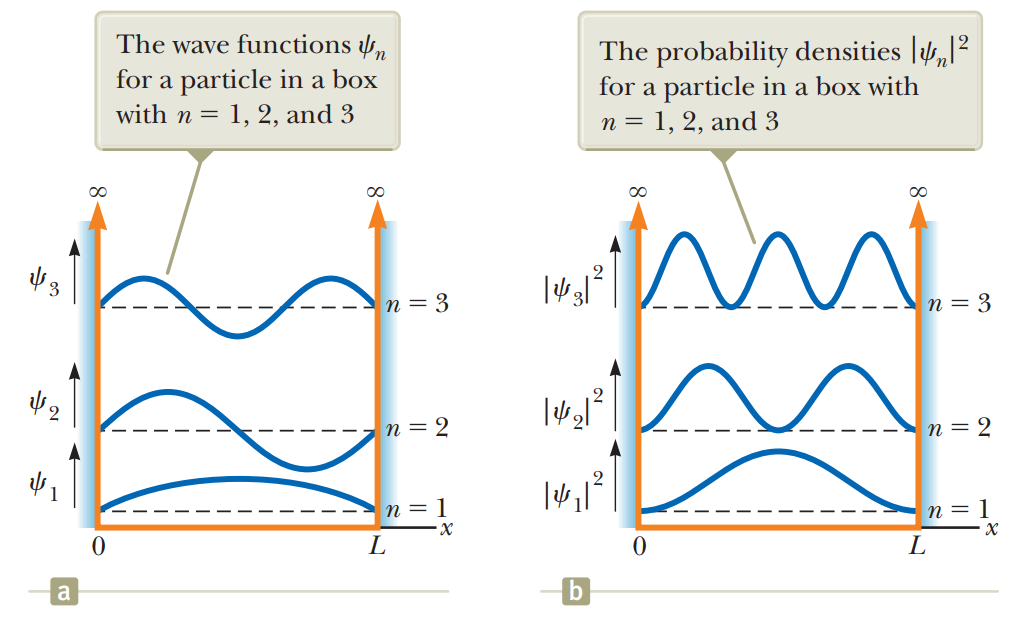
\includegraphics[width=0.75\textwidth]{assets/psi-in-box.png}
	\caption{\(\psi\) and \({\ab|\psi|}^2\) for particle in box}
	\label{fig:psi-in-box}
\end{figure}
This also means that the particle can only take on \it{allowed momenta}:
\[p_n = \f{h}{\lambda_n} = \f{nh}{2L}\]

\begin{marginfigure}
	\centering
	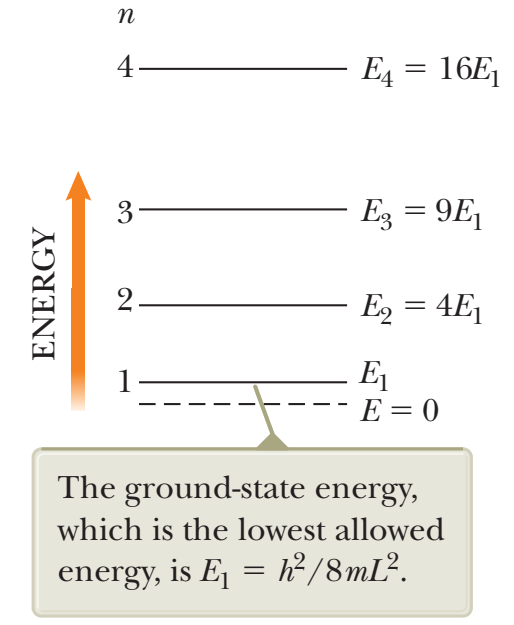
\includegraphics[width=.8\textwidth]{assets/energy-levels.png}
	\caption{Allowed energy levels}
	\label{fig:energy-levels}
\end{marginfigure}
And therefore, the particle can only take on \it{allowed energies}, which are quantised:
\[E_n = K_n = \f{p_n^2}{2m} = \f{n^2h^2}{8mL^2}\]

Electrons can transition between any two energy levels, so
the number of \it{allowed transitions} is \({}^nC_2\) for \(n\) energy levels.

\begin{definition}{Ground state}{ground-state}
	The lowest possible energy state of the atom, where \(n = 1\).
\end{definition}

\section{Line spectra}

\begin{definition}{Excitation}{excitation}
	The absorption of a photon by one \ce{e-} to promote
	the electron from a lower allowed energy level to a higher allowed energy level.
	\[hf = E_\text{hi} - E_\text{lo}\]
\end{definition}
\(\therefore\;\) The energy of the photon must be \it{exactly} the energy
difference \(\Delta E\).

Light may be emitted by atoms when electrons de-excite.
The light is not observed as a continuous spectrum of wavelengths,
but appears as a series of discrete lines at specific wavelengths.
\begin{definition}{De-excitation}{deexcitation}
	The release of energy by one \ce{e-} \it{in the form of a photon}
	when it moves from a higher energy level to a lower energy level.
	\[hf = E_\text{hi} - E_\text{lo}\]
\end{definition}

\begin{definition}{Ionisation}{ionisation}
	The absorption of sufficient energy by an electron
	to completely leave the atom.
\end{definition}

\subsection{Emission spectra}
\begin{marginfigure}
	\centering
	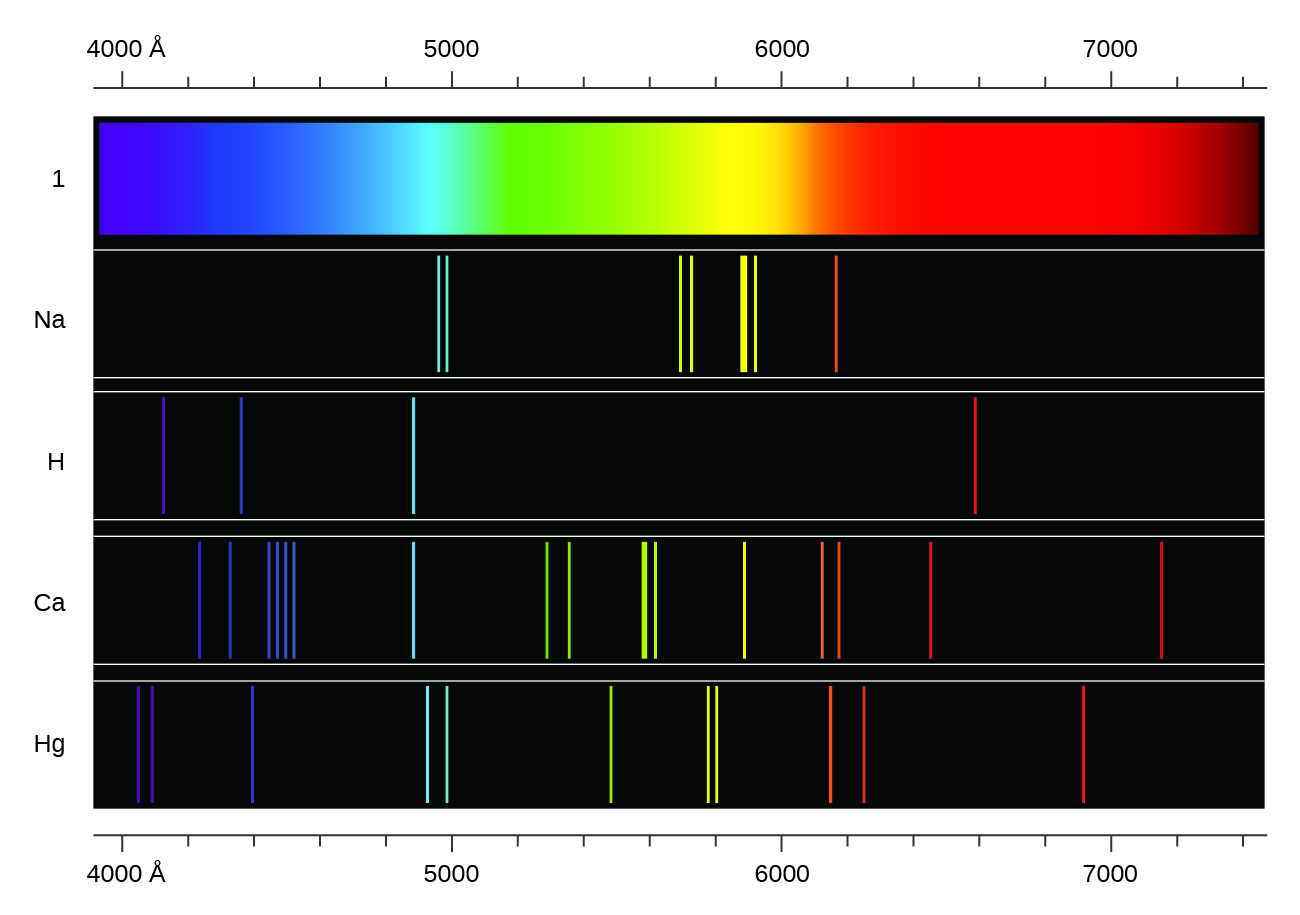
\includegraphics[width=\textwidth]{assets/atomic-spectra.jpg}
	\caption{Emission spectra of \ce{Na}, \ce{H}, \ce{Ca} and \ce{Hg}}
	\label{fig:emission-spectra}
\end{marginfigure}
When e.m.~radiation is incident on atoms, \ce{e-} can become excited.

Atoms collide with fast-moving electrons in a discharge tube,
causing part of the free electrons' k.e.~to be transferred to the atoms.
The \it{bound electrons} in the atoms excite.

When the excited atoms de-excite, the bound electrons return to a lower
energy level and each emit one photon.
\[hf = E_{\text{photon}} = E_\text{hi} - E_\text{lo}\]
This produces emission spectra (\cref{fig:emission-spectra}).

\subsection{Absorption line spectra}
Light of a \it{continuous spectrum} of wavelengths passes through a
\underline{cool gas} at \underline{low pressure}.

Photons whose energies match the energy difference
between ground state and an excited state are absorbed;
these photons are removed from the light.

\begin{marginfigure}
	\centering
	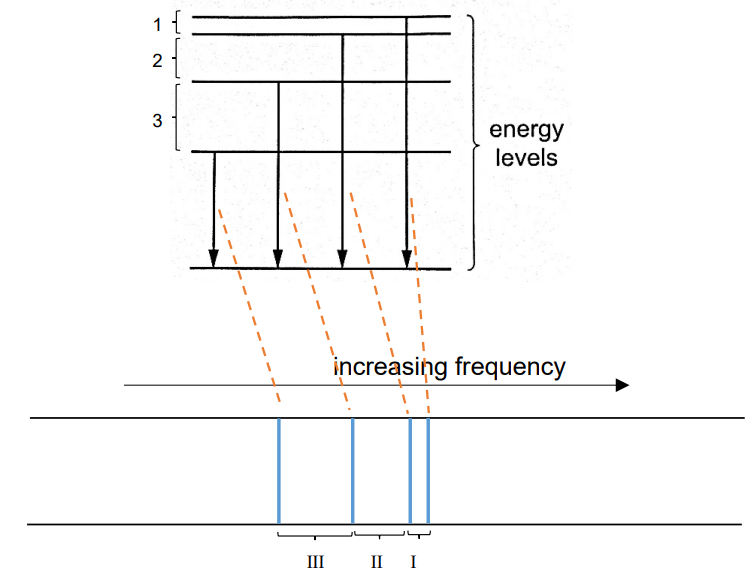
\includegraphics[width=\textwidth]{assets/absorption-spectra.png}
	\caption{Absorption line spectrum}
	\label{fig:absorption-spectra}
\end{marginfigure}
Although the atoms in the gas release photons
when they eventually de-excite,
\begin{itemize}
	\item the \it{released photons are radiated in all directions}; they may not reach the observer
	\item de-excitation may happen through \it{intermediate transitions}, so the emitted photons may have different energies from the original incident photons.
\end{itemize}
The resultant intensity of these select photons decreases \(\implies\)
appear as dark lines.
Since \(\Delta E \propto f\), the spacing between lines
is proportional to the energy gap involved in allowed transitions.
